% ------------------------------------------------------------
% SmartGate - Proyecto integrador 3
% Versión reordenada del informe. Compilar con XeLaTeX o LuaLaTeX
% (usa fontspec).
% ------------------------------------------------------------

\documentclass[a4paper,12pt]{report}
\usepackage{fontspec}
\usepackage[spanish,es-tabla,es-noshorthands]{babel}
\usepackage{graphicx}
\usepackage{geometry}
\usepackage{titlesec}
\usepackage{fancyhdr}
\usepackage{indentfirst}
\usepackage{caption}
\usepackage{subcaption}
\usepackage{array}
\usepackage{float}
\usepackage{tikz}
\usetikzlibrary{positioning,arrows.meta,babel}
\usepackage{amsmath}
\usepackage{amssymb}
\usepackage{hyperref}

% Numero de pagina a la derecha
\fancyhf{}
\renewcommand{\headrulewidth}{0pt}
\fancyfoot[R]{\thepage}
\pagestyle{fancy}
\fancypagestyle{plain}{
  \fancyhf{}
  \renewcommand{\headrulewidth}{0pt}
  \fancyfoot[R]{\thepage}
}

% Eliminar titulo de capitulo por defecto
\titleformat{\chapter}[display]
{\normalfont\bfseries}{}{0pt}{\Huge}

\titleformat{\subsection}
{\normalfont\large\bfseries}{\hspace{2em}\thesubsection}{1em}{}

% Disminuir margen de titulo
\titlespacing*{\chapter}{0pt}{-50pt}{0pt}
\titlespacing*{\section}{0pt}{0pt}{0pt}
\titlespacing*{\subsection}{0pt}{0pt}{0pt}

% Normas de párrafos
\renewcommand{\baselinestretch}{1.5}
\setlength{\parskip}{12pt}

% Margenes de documento
\newgeometry{
    top=2.5cm,
    bottom=2.5cm,
    outer=2.5cm,
    inner=2.5cm,
    includefoot,
    footskip=1.5cm
}

% Estilos comunes para los diagramas de bloques
\tikzset{
    caja/.style={rectangle, draw=black, align=center, text width=8.5cm, inner sep=6pt, font=\normalsize},
    cajachica/.style={rectangle, draw=black, align=center, text width=4.6cm, inner sep=6pt, font=\normalsize},
    flecha/.style={-{Stealth}, thick},
    dflecha/.style={{Stealth}-{Stealth}, thick},
    etiqueta/.style={font=\footnotesize, align=center, fill=white, inner sep=2pt}
}

\hyphenation{e-jem-plo es-pe-ci-fí-cas ge-ne-ra-ti-va com-pues-ta par-ti-cu-lar cus-to-mi-za-ble de-sa-rro-llar res-pon-de-rá di-fe-ren-tes co-rres-pon-dien-te au-to-ma-ti-za-da se-pa-ra-da se-pa-ran-do per-te-ne-cien-tes es-ca-la-bles se-pa-rar}

\begin{document}

\begin{center}
\thispagestyle{empty}
    % Logo ORT
    \begin{figure}
        \centering
        
\includegraphics[scale=1.2]{Imagenes/ortlogo.png}
        \vspace{2cm}
    \end{figure}

    \Huge
    \textbf{SmartGate}

   \Large
   - Proyecto integrador 3

   \vspace{1.7cm}

   Ingeniería en Electrónica, Universidad ORT Uruguay

   \vspace{1cm}

    \textbf{Mateo Menchaca - 251812}

    \textbf{Mateo Silva - 282489}

   \vspace{0.4cm}

   \vfill
   \large
   2026

\end{center}


\tableofcontents

\chapter{Descripción general del sistema}

\section{Función general}

La Raspberry Pi constituye el controlador principal de SmartGate. En ella se ejecuta una aplicación desarrollada en Python que integra la cámara, los modelos, la lógica de autorización, las entradas y salidas GPIO y la comunicación con Supabase. Esta elección permite realizar localmente las decisiones críticas: la detección, la validación de vida, el reconocimiento facial y la apertura del portón no dependen de que exista una conexión permanente a Internet.

\section{Componentes del sistema y su interacción}

El sistema se compone de cuatro bloques: la interfaz web de administración, la base de datos en Supabase, la Raspberry Pi que realiza el reconocimiento y la interfaz electrónica que actúa sobre el portón. La interfaz web y la Raspberry Pi trabajan sobre la misma fuente de datos: cuando un usuario es creado o actualizado desde la web, la modificación queda almacenada en Supabase y puede ser consultada por la Raspberry Pi. En sentido inverso, los eventos enviados por el dispositivo quedan disponibles en la interfaz para su supervisión. La figura~\ref{fig:interaccion} resume esta interacción.

\begin{figure}[H]
    \centering
    \begin{tikzpicture}[node distance=1.5cm]
        \node[caja] (web) {\textbf{Interfaz web}\\ Administración de usuarios\\ Carga de imágenes y consultas};
        \node[caja, below=of web] (supa) {\textbf{Supabase}\\ Base de datos PostgreSQL\\ Almacenamiento y eventos};
        \node[caja, below=of supa] (rpi) {\textbf{Raspberry Pi}\\ Reconocimiento facial\\ Procesamiento y decisión};
        \node[caja, below=of rpi] (sg) {\textbf{SmartGate}\\ Interfaz electrónica\\ Control de acceso físico};
        \draw[dflecha] (web) -- node[etiqueta]{API y consultas} (supa);
        \draw[dflecha] (supa) -- node[etiqueta]{API HTTPS: usuarios y registros} (rpi);
        \draw[dflecha] (rpi) -- node[etiqueta]{Orden de apertura y estado del portón} (sg);
    \end{tikzpicture}
    \caption{Interacción entre la interfaz web, Supabase, la Raspberry Pi y el sistema de acceso.}
    \label{fig:interaccion}
\end{figure}

Cada uno de estos bloques se desarrolla en los capítulos siguientes: la interfaz con el portón en el capítulo~\ref{cap:interfaz}, los modelos de reconocimiento en el capítulo~\ref{cap:modelos}, el programa de la Raspberry Pi en el capítulo~\ref{cap:programa} y la base de datos, la interfaz web y el funcionamiento sin conexión en el capítulo~\ref{cap:datos}.

\section{Organización del desarrollo}

El desarrollo de SmartGate se realizó de forma escalonada. Desde el inicio se separó el trabajo en dos niveles: un producto mínimo viable (MVP), encargado de demostrar el funcionamiento principal del sistema, y un conjunto de funcionalidades adicionales que solamente se abordarían una vez que el núcleo estuviera integrado y probado. Esta separación permitió mantener un objetivo funcional durante todo el proyecto y evitó que las mejoras opcionales comprometieran la entrega principal.

El trabajo comenzó con la investigación de modelos de detección facial, reconocimiento y antispoofing, junto con el análisis de la Raspberry Pi, la cámara y la electrónica necesaria para interactuar con el portón. A partir de esa investigación se definió una arquitectura modular y se utilizaron modelos previamente entrenados para construir una primera versión del pipeline. Luego se incorporó el control físico y, una vez validado el ciclo completo, se avanzó sobre la base de datos, la interfaz web, la persistencia offline y las herramientas relacionadas con el entrenamiento de modelos propios.

\begin{figure}[H]
    \centering
    \begin{tikzpicture}[
        phase/.style={rectangle, rounded corners, draw=black, thick, align=center, text width=2.55cm, minimum height=1.45cm, font=\small, fill=blue!8},
        extra/.style={rectangle, rounded corners, draw=black, thick, align=center, text width=2.55cm, minimum height=1.45cm, font=\small, fill=green!10},
        pending/.style={rectangle, rounded corners, draw=black, thick, align=center, text width=2.55cm, minimum height=1.45cm, font=\small, fill=orange!15}
    ]
        \node[phase] (research) at (0,0) {Investigación\\ y definición};
        \node[phase] (mvp) at (3.8,0) {Implementación\\ del MVP};
        \node[extra] (extras) at (7.6,0) {Extras\\ operativos};
        \node[pending] (training) at (11.4,0) {Dataset y\\ entrenamiento};

        \draw[flecha] (research) -- (mvp);
        \draw[flecha] (mvp) -- (extras);
        \draw[flecha] (extras) -- (training);
    \end{tikzpicture}
    \caption{Desarrollo escalonado de SmartGate. La última etapa se inició, pero no pudo completarse.}
    \label{fig:desarrollo-escalonado}
\end{figure}

La figura~\ref{fig:desarrollo-escalonado} resume las etapas: investigación y definición de la arquitectura, el hardware y los modelos; implementación del MVP, que comprende el pipeline y el control físico; extras operativos, como Supabase, la interfaz web y la persistencia; y finalmente el dataset y el entrenamiento propio, etapa que se inició pero no se completó. El detalle de lo implementado en cada nivel se presenta en el capítulo~\ref{cap:desarrollo}.

\chapter{Interfaz con el portón}
\label{cap:interfaz}

El desarrollo del módulo de control físico requiere definir previamente qué tipo de señales pueden considerarse disponibles en un automatismo residencial representativo. Para ello se analizaron distintas centrales utilizadas en portones corredizos, principalmente de las marcas PPA y SEG, buscando identificar características comunes en la forma de accionar el portón, detectar sus posiciones extremas y alimentar dispositivos auxiliares.

El objetivo de este análisis no es seleccionar una única central como requisito del proyecto, sino establecer una base suficientemente representativa a partir de controladores de uso común. De esta manera, el desarrollo posterior de la interfaz electrónica podrá realizarse sobre señales y modos de operación que aparecen de forma recurrente en distintos equipos, evitando depender desde el inicio de una implementación particular.

\section{Controladores considerados}

Entre las centrales analizadas se encuentra la PPA Triflex Facility, utilizada en distintas líneas de automatizadores de la marca. Su documentación contempla entradas destinadas a finales de carrera y a botoneras externas, además de una alimentación auxiliar disponible para accesorios. Para el final de carrera, la central interpreta el accionamiento cuando la entrada correspondiente es llevada a GND, mientras que la orden proveniente de una botonera se implementa mediante el cierre de contactos sobre las entradas de mando correspondientes.

También se consideraron controladores correspondientes a la familia PPA Pop Connect. Estos equipos mantienen una arquitectura similar desde el punto de vista funcional, al disponer de entradas para el accionamiento externo y de señales destinadas a determinar la posición del portón. La implementación interna y los niveles eléctricos pueden variar respecto de otras centrales, por lo que su consideración resulta útil para no asociar el posterior diseño a un único valor de tensión o a una única disposición de conectores.

Dentro de los automatismos SEG se analizaron principalmente las centrales Wave y G-II. La central Wave dispone de entradas de botonera referenciadas al GND del controlador y de una salida auxiliar de 12~Vcc, limitada a una corriente especificada por el fabricante. Esto permite observar que, además de las señales de mando, existen controladores que proporcionan alimentación destinada a dispositivos externos dentro del mismo dominio eléctrico de la placa.

La central SEG G-II presenta una estructura comparable, con entradas destinadas al accionamiento mediante botonera y una salida auxiliar de 12~Vcc. En este caso la documentación especifica una capacidad de corriente superior y señala que dicha salida no se encuentra regulada, mostrando que la disponibilidad de alimentación auxiliar no implica necesariamente características eléctricas idénticas entre diferentes controladores.

También se tomó como referencia la línea SEG Solo CH, donde el posicionamiento del portón se resuelve mediante sensores magnéticos asociados a los extremos del recorrido. La documentación de esta familia describe el uso de sensores reed normalmente abiertos para la detección de los finales de carrera, confirmando la presencia de una lógica basada en el cambio de estado de un contacto asociado a una entrada de la central.

El análisis conjunto de estos controladores permite identificar una estructura funcional común, aun cuando existan diferencias en tensión, capacidad de corriente, tipo de sensor y disposición física de los terminales.

\section{Señales disponibles en las centrales}

\subsection{Final de carrera}

Para SmartGate resulta necesario conocer si el portón se encuentra completamente cerrado antes de generar una nueva orden de apertura. En lugar de incorporar un sensor de posición independiente, se toma como base el aprovechamiento del sistema de final de carrera ya presente en el automatismo.

En las centrales analizadas, la posición extrema se determina a partir del cambio de estado de una entrada asociada al sensor de final de carrera. En diferentes implementaciones este sensor puede encontrarse constituido por un contacto mecánico, un relé o un sensor magnético reed, pero funcionalmente la central recibe una modificación de nivel eléctrico cuando el portón alcanza la posición correspondiente.

Como representación general, se considerará una entrada de referencia asociada al final de carrera y referenciada al GND de la central. Entre dicha entrada y GND se encuentra el contacto seco del sensor. Cuando este contacto permanece abierto, sobre la entrada puede existir una tensión de control determinada por la electrónica interna del controlador, o bien presentarse un estado de alta impedancia. Al accionarse el final de carrera, el contacto cierra el circuito y establece la conexión de dicha entrada hacia GND.

De forma conceptual:

\begin{center}
\texttt{REF\_FC} $\rightarrow$ contacto de final de carrera $\rightarrow$ \texttt{GND}
\end{center}

El valor de tensión presente en \texttt{REF\_FC} con el contacto abierto no se considerará único, dado que depende de la electrónica interna de cada controlador. En los equipos analizados aparecen diferentes niveles de alimentación y arquitecturas, por lo que esta entrada podrá encontrarse polarizada a un determinado nivel de control o permanecer en alta impedancia. En consecuencia, esta señal se tratará posteriormente como una variable de interfaz y no como un nivel lógico fijo.

Para el proyecto únicamente interesa recuperar la información correspondiente al final de carrera de cierre. De esta manera, SmartGate podrá conocer el estado físico del portón utilizando el mismo elemento que emplea la central original para determinar que el recorrido de cierre ha finalizado.

\subsection{Accionamiento del portón}

La segunda señal de interés corresponde al comando utilizado para solicitar un movimiento del portón. Los controladores considerados disponen de entradas destinadas a botoneras, pulsadores o dispositivos externos, permitiendo actuar sobre el automatismo sin intervenir directamente en su etapa de potencia.

En términos funcionales, estas entradas operan mediante el cierre temporal de un contacto entre la entrada de mando y la referencia de GND de la central. Este comportamiento es equivalente al producido por una botonera convencional instalada en paralelo con otros medios de accionamiento.

Como representación general se considerará:

\begin{center}
\texttt{BTN} $\rightarrow$ contacto temporal $\rightarrow$ \texttt{GND}
\end{center}

La utilización de esta entrada resulta especialmente conveniente para SmartGate porque permite que el sistema externo únicamente genere una solicitud de accionamiento. La interpretación de dicha solicitud, la secuencia de movimiento del motor, la actuación de los finales de carrera y las demás funciones propias del automatismo continúan siendo gestionadas por la central original.

De esta forma, la integración se realiza sobre una interfaz que ya ha sido prevista por el fabricante para mandos externos, sin necesidad de actuar directamente sobre relés de potencia, bobinados del motor u otros elementos internos del controlador.

\subsection{Alimentación auxiliar}

Otro aspecto observado durante el análisis es la disponibilidad de salidas auxiliares de alimentación en distintas centrales. Estas salidas se utilizan habitualmente para alimentar fotocélulas, receptores, sensores u otros accesorios asociados al automatismo.

En la central PPA Triflex Facility se dispone de una salida auxiliar de 15~Vcc, mientras que en las centrales SEG Wave y SEG G-II aparecen salidas de 12~Vcc con diferentes capacidades de corriente. Esto muestra que es frecuente disponer dentro de la propia central de una fuente de continua referenciada a su GND, aunque sus características concretas dependen del modelo utilizado.

La existencia de este tipo de alimentación resulta relevante para el desarrollo posterior, ya que permite considerar la posibilidad de alimentar la electrónica asociada al lado del portón desde el propio dominio eléctrico de la central. Sin embargo, la tensión disponible, su regulación y la corriente máxima deberán considerarse individualmente para cada controlador.

\section{Base adoptada para el diseño}

A partir de las centrales estudiadas se tomará como base una arquitectura en la que el portón dispone de una referencia eléctrica común asociada a su controlador, una señal de final de carrera de cierre y una entrada destinada al accionamiento mediante botonera.

La detección de portón cerrado se realizará a partir del cambio de estado de la señal utilizada por el propio final de carrera, mientras que la orden de movimiento se generará reproduciendo eléctricamente el comportamiento de un pulsador externo entre la entrada de mando y GND.

Asimismo, se considerará posible la existencia de una alimentación auxiliar dentro del dominio eléctrico de la central, con valores que pueden encontrarse aproximadamente en el entorno de 12 a 15~Vcc según el controlador utilizado.

Estas condiciones establecen la base funcional y eléctrica sobre la cual se desarrolla la interfaz de SmartGate, cuyo circuito de lectura del final de carrera y su implementación en placa se describen a continuación.

\section{Interfaz de lectura del final de carrera}

La lectura del estado del final de carrera se plantea mediante una interfaz conectada en paralelo con la señal original del portón, procurando que su incorporación no modifique el funcionamiento normal del controlador. El circuito actúa de esta forma como un \textit{sniffer} de la señal asociada al contacto magnético, limitando la corriente intercambiada con la entrada original y manteniendo aislada eléctricamente la Raspberry Pi respecto de la electrónica del automatismo.

Para el diseño se consideran dos posibles comportamientos de la entrada de final de carrera cuando el contacto se encuentra abierto. En el primer caso, la controladora puede incorporar internamente una resistencia de pull-up, manteniendo el pin a una tensión lógica propia. En el segundo, la entrada puede permanecer en un estado de alta impedancia, dependiendo exclusivamente del cierre del contacto hacia masa para detectar el final de carrera. En ambos casos, al accionarse el sensor, la señal se establece próxima a GND.

Con el objetivo de contemplar ambas posibilidades sin imponer directamente la tensión de alimentación sobre una entrada cuya electrónica interna es desconocida, se incorpora una polarización débil hacia aproximadamente 3,3~V. Esta tensión se obtiene a partir de la menor alimentación prevista para la controladora, $V_{CC} = 12$~V, mediante un divisor resistivo de elevada impedancia. Si la tensión disponible en el automatismo fuera superior, deberá acondicionarse previamente para conservar este mismo nivel de polarización.

La elevada resistencia equivalente del divisor hace que, cuando la controladora posee un pull-up propio, sea principalmente la electrónica original la que determine la tensión del nodo. Por ejemplo, frente a resistencias internas del orden de 10~k$\Omega$ a 47~k$\Omega$, una red externa con una resistencia equivalente cercana a 100~k$\Omega$ introduce únicamente una carga reducida y no modifica de forma significativa el nivel lógico establecido por la placa. En cambio, si la entrada se encuentra en alta impedancia, esta misma red fija el nodo en torno a 3,3~V, evitando que la entrada del comparador quede flotante. De esta forma se obtiene un comportamiento definido para ambas arquitecturas sin aplicar directamente 12~V sobre el pin de final de carrera.

La señal obtenida se compara con una referencia de aproximadamente 1,3~V. Mientras el contacto permanece abierto, la entrada se mantiene por encima de este umbral, ya sea debido a la polarización interna de la controladora o a la red auxiliar de 3,3~V. Cuando el final de carrera conecta la señal a masa, la tensión desciende por debajo de la referencia y el comparador conmuta. Para esta función se prevé utilizar un LM393, cuya salida de colector abierto permite controlar directamente la corriente del LED de un optoacoplador.

La salida del comparador gobierna un PC817 mediante una resistencia serie de 1,5~k$\Omega$. El transistor de salida del optoacoplador pertenece a un circuito eléctricamente independiente, alimentado a 3,3~V desde el lado de la Raspberry Pi. En este sector se utiliza una resistencia de pull-up de 3,3~k$\Omega$, de forma que el estado de conducción del PC817 se transforma en un nivel lógico adecuado para una entrada GPIO.

Esta separación mediante optoacoplador evita compartir la referencia de masa entre el controlador del portón y la Raspberry Pi. De esta forma, cualquier diferencia de potencial, ruido o perturbación presente en la electrónica de potencia queda desacoplada del sistema de procesamiento. En conjunto, la elevada impedancia de la etapa de sensado y el aislamiento óptico permiten obtener información del final de carrera con una influencia mínima sobre el circuito original y sin establecer una conexión eléctrica directa con la Raspberry Pi.

\section{Implementación de la placa de interfaz}

A partir del análisis de las señales disponibles se diseñó y fabricó una placa de circuito impreso (PCB) por parte del equipo en las instalaciones de la Universidad ORT Uruguay. La placa concentra en una única solución las conexiones necesarias para vincular la Raspberry Pi con la central del portón, los finales de carrera, los indicadores y los actuadores. El uso de borneras facilita el montaje y el mantenimiento, mientras que los zócalos permiten reemplazar componentes sin intervenir directamente sobre las pistas.

Esta implementación permitió pasar del esquema conceptual a un módulo físico reproducible y ordenado. Además de reducir conexiones sueltas durante las pruebas, la PCB establece puntos de entrada y salida definidos, simplifica el diagnóstico y deja una base adecuada para futuras revisiones del hardware.

\begin{figure}[H]
    \centering
    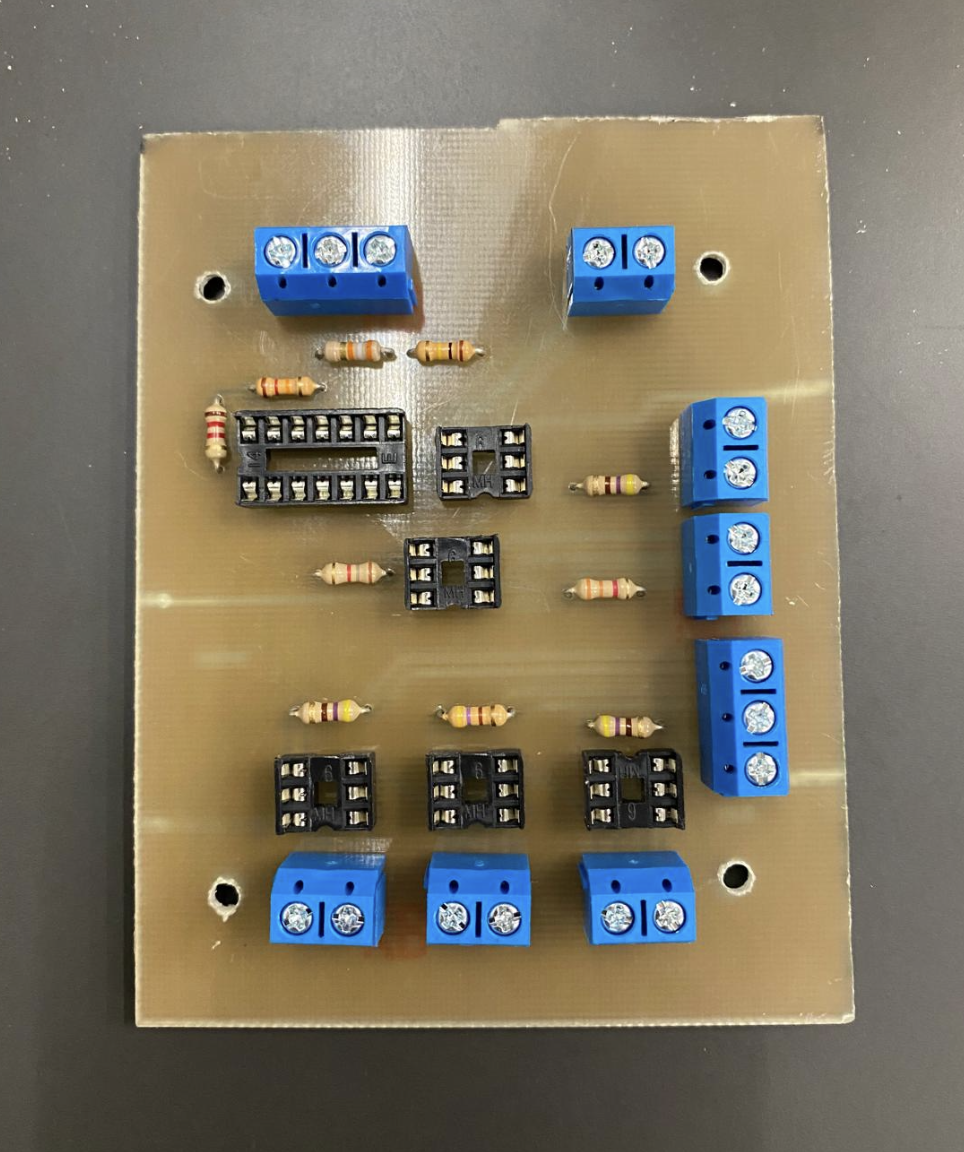
\includegraphics[width=0.6\textwidth]{Imagenes/pcb_interfaz.png}
    \caption{PCB de interfaz desarrollada y fabricada por el equipo en la Universidad ORT Uruguay.}
    \label{fig:pcb}
\end{figure}

\chapter{Modelos de machine learning}
\label{cap:modelos}

El procesamiento facial de SmartGate se dividió en tres etapas, cada una orientada a resolver un problema diferente. En primer lugar, YuNet localiza el rostro dentro de la imagen y obtiene la información necesaria para prepararlo. Luego, MiniFASNetV2 evalúa si la muestra presenta características correspondientes a un rostro real o a un intento de suplantación. Finalmente, SFace genera una representación del rostro que permite compararlo con los usuarios registrados.

Esta separación permite utilizar un modelo especializado para cada función y evitar que las etapas de mayor costo se ejecuten sobre imágenes que no resulten adecuadas. Utilizar menos modelos implicaría eliminar alguna de las verificaciones necesarias para la autenticación, mientras que incorporar nuevas redes sin una función diferenciada aumentaría el tiempo de procesamiento y la complejidad de la decisión.

\section{YuNet: detección facial}

\subsection{Elección del modelo}

Se seleccionó YuNet como detector facial de SmartGate debido a que permite localizar rostros mediante una arquitectura compacta y obtener, en una misma inferencia, la información necesaria para preparar las muestras utilizadas posteriormente. Al encontrarse al comienzo del pipeline, esta etapa debe ejecutarse sobre las imágenes provenientes de la cámara antes de conocer si contienen un rostro válido, por lo que resulta conveniente que el procesamiento requerido sea reducido.

El bajo costo computacional de YuNet responde a un diseño orientado a dispositivos con recursos limitados. Su arquitectura combina una red pequeña de extracción de características con una estructura simplificada para integrar información de diferentes escalas. Estas decisiones reducen la cantidad de parámetros que deben almacenarse y el trabajo necesario para procesar cada imagen. En SmartGate, esto favorece la ejecución repetida del detector y permite reservar recursos para las etapas posteriores de verificación de autenticidad y reconocimiento facial. La extracción y combinación de características se explican en el apartado de funcionamiento.

Otro motivo de elección es que YuNet proporciona tanto la ubicación del rostro como los puntos de referencia necesarios para su posterior alineamiento. Disponer de ambas salidas en una misma inferencia evita incorporar un modelo adicional dedicado exclusivamente a localizar estos puntos y simplifica la preparación de las muestras.

La utilización de un detector independiente resulta necesaria porque MiniFASNetV2 y SFace trabajan sobre regiones faciales y no tienen como objetivo buscar personas dentro de una escena completa. YuNet cubre esta necesidad y permite que cada modelo posterior se concentre en su tarea específica.

\subsection{Funcionamiento del modelo}

El flujo comienza con una imagen proveniente de la cámara, que se entrega como entrada a YuNet. Su red convolucional aplica filtros aprendidos durante el entrenamiento para extraer características útiles para la detección facial. Este proceso genera mapas de características con distintas resoluciones espaciales, que representan la información de la imagen a diferentes escalas.

A continuación, una estructura simplificada de pirámide de características combina información de distintos niveles de la red. Esto permite aprovechar tanto detalles espaciales como patrones más generales y facilita la detección de rostros de diferentes tamaños. La extracción y la combinación de características forman parte de una misma inferencia.

A partir de estas representaciones, el modelo genera detecciones candidatas. Cada una contiene un cuadro delimitador (\textit{bounding box}), una puntuación de confianza y cinco puntos de referencia faciales (\textit{landmarks}), correspondientes a los dos ojos, la nariz y las dos comisuras de la boca. El cuadro indica la ubicación y el tamaño del rostro, mientras que la confianza permite valorar la detección. Esta puntuación no determina la identidad de la persona ni la autenticidad del rostro.

Las predicciones pasan luego por una etapa de posprocesamiento. Primero se descartan las candidatas cuya confianza se encuentra por debajo del umbral configurado. Después se aplica supresión de no máximos (\textit{Non-Maximum Suppression}, NMS), que prioriza las detecciones de mayor confianza y elimina aquellas que se superponen excesivamente con ellas. De esta manera, se reducen las detecciones repetidas sobre un mismo rostro.

El detector devuelve las detecciones conservadas junto con sus cuadros delimitadores, puntuaciones de confianza y puntos faciales. Si ninguna candidata supera el filtrado, el resultado no contiene rostros detectados.

Las etapas posteriores del pipeline utilizan esta información para preparar las muestras. El cuadro delimitador permite localizar la región facial que se debe recortar, mientras que los puntos de referencia permiten calcular el alineamiento previo al reconocimiento. Este último ajusta la posición, la escala y la inclinación del rostro en el plano de la imagen. El recorte y el alineamiento son operaciones posteriores a la detección realizada por YuNet.

\subsection{Diagrama de flujo del modelo}

\begin{figure}[H]
    \centering
    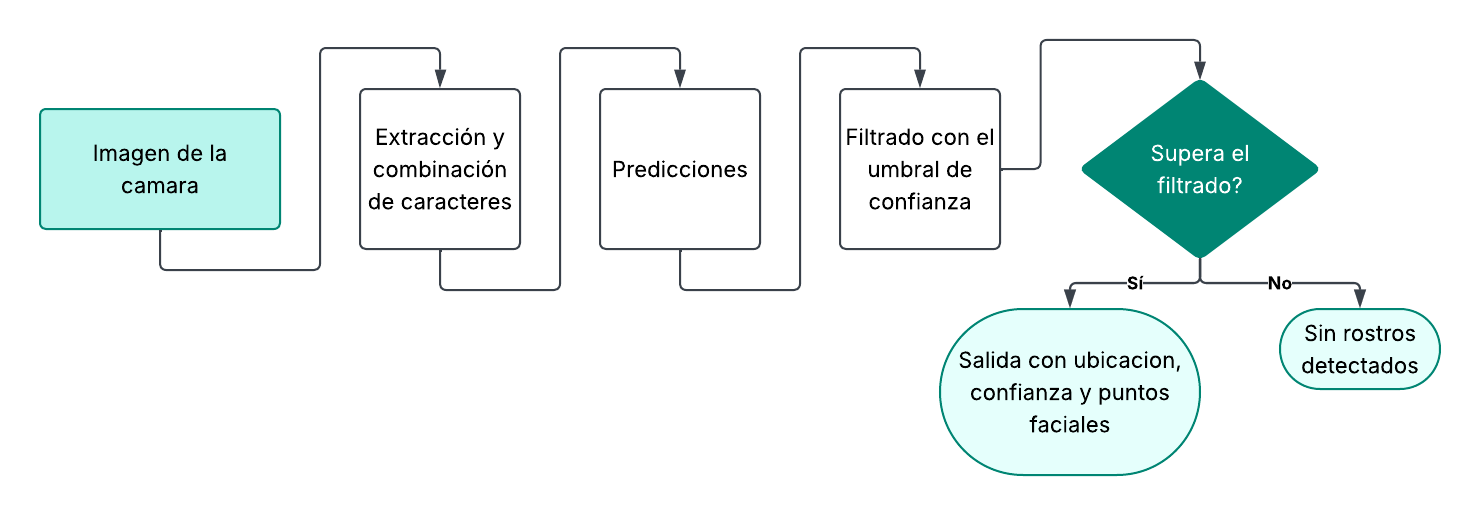
\includegraphics[width=\textwidth]{Imagenes/flujo_yunet.png}
    \caption{Diagrama de flujo de YuNet.}
    \label{fig:flujo-yunet}
\end{figure}

\section{MiniFASNetV2: antispoofing}

\subsection{Elección del modelo}

Se seleccionó MiniFASNetV2 para la detección de intentos de suplantación debido a que la identificación de una persona por sí sola no permite determinar si el rostro observado proviene de una persona físicamente presente. Una fotografía impresa o una imagen mostrada en una pantalla puede conservar suficientes características de identidad para ser reconocida. Por este motivo, antes de utilizar el resultado de SFace para autorizar un acceso se incorpora una etapa independiente de anti-spoofing.

MiniFASNetV2 pertenece a una familia de redes diseñadas específicamente para esta tarea y desarrolladas a partir de una arquitectura basada en MobileFaceNet. Su tamaño reducido responde a la aplicación de poda de canales, que disminuye la cantidad de información intermedia que debe procesar la red y, con ello, sus parámetros y operaciones. Además, utiliza bloques que combinan convoluciones por canal y convoluciones puntuales, permitiendo extraer características con un costo menor que el de convoluciones convencionales equivalentes. El funcionamiento de estos bloques se explica en el apartado siguiente.

Estas características resultan convenientes para SmartGate porque permiten agregar una evaluación de autenticidad sin introducir una red de gran tamaño en el pipeline. Esto favorece el procesamiento frecuente de muestras faciales y deja recursos disponibles para la detección y el reconocimiento. Asimismo, el modelo analiza imágenes sin requerir que la persona complete una secuencia de acciones, lo que permite incorporar la comprobación al flujo de acceso sin solicitar gestos adicionales.

MiniFASNetV2 se utiliza como único modelo para esta etapa porque agrega una comprobación que ni YuNet ni SFace realizan. Eliminarlo permitiría que una muestra correctamente detectada e identificada avanzara sin evaluar su autenticidad, mientras que utilizar varios clasificadores de anti-spoofing obligaría a realizar inferencias adicionales y combinar sus resultados. Su elección permite incorporar esta segunda condición de seguridad manteniendo una etapa específicamente dedicada a detectar intentos de suplantación.

La separación respecto del reconocimiento también permite ajustar el criterio de aceptación del anti-spoofing sin modificar la comparación de identidades realizada por SFace.

\subsection{Funcionamiento del modelo}

El flujo comienza con la imagen de la cámara y la ubicación del rostro obtenida mediante YuNet. A partir de esta información se prepara un recorte facial, conservando el contexto alrededor del rostro que requiera la versión del modelo utilizada. Luego se ajusta el recorte al tamaño de entrada correspondiente y se convierte en un tensor, es decir, una representación numérica organizada que la red puede procesar. Esta preparación debe respetar las condiciones de entrada previstas durante el entrenamiento.

La muestra atraviesa una serie de bloques convolucionales que extraen características visuales aprendidas para distinguir rostros reales de representaciones utilizadas como ataque. Dentro de estos bloques, las convoluciones por canal (\textit{depthwise}) procesan por separado cada canal de características, mientras que las convoluciones puntuales de $1 \times 1$ combinan información entre canales. Esta separación reduce el cálculo necesario para transformar las representaciones internas.

La red también incorpora conexiones residuales, que suman la entrada de determinados bloques a su salida y facilitan la propagación de información. A medida que avanza el procesamiento, se reduce la resolución espacial de los mapas de características hasta obtener una representación compacta de la muestra.

Esta representación se entrega a una capa de clasificación, que produce una puntuación sin normalizar, denominada \textit{logit}, para cada clase considerada durante el entrenamiento. En la implementación de referencia, estas puntuaciones se transforman mediante la función \textit{softmax}, obteniendo valores entre cero y uno cuya suma es uno. Estos valores expresan la preferencia relativa del clasificador por cada clase.

La interpretación de la salida permite distinguir la clase correspondiente a una muestra real de las asociadas a ataques. Sobre estas puntuaciones, la aplicación aplica su criterio de aceptación del anti-spoofing. La clasificación y el criterio de aceptación constituyen pasos diferentes: la red produce puntuaciones y la lógica del sistema determina si resultan suficientes para aceptar la muestra.

Si el criterio no se cumple, la muestra no supera esta comprobación. Si se cumple, queda satisfecha la condición de anti-spoofing, cuyo resultado se combina con la evaluación de identidad realizada mediante SFace. Por lo tanto, la salida de MiniFASNetV2 aporta una estimación de autenticidad y no constituye, por sí sola, una autorización de acceso.

\subsection{Diagrama de flujo del modelo}

\begin{figure}[H]
    \centering
    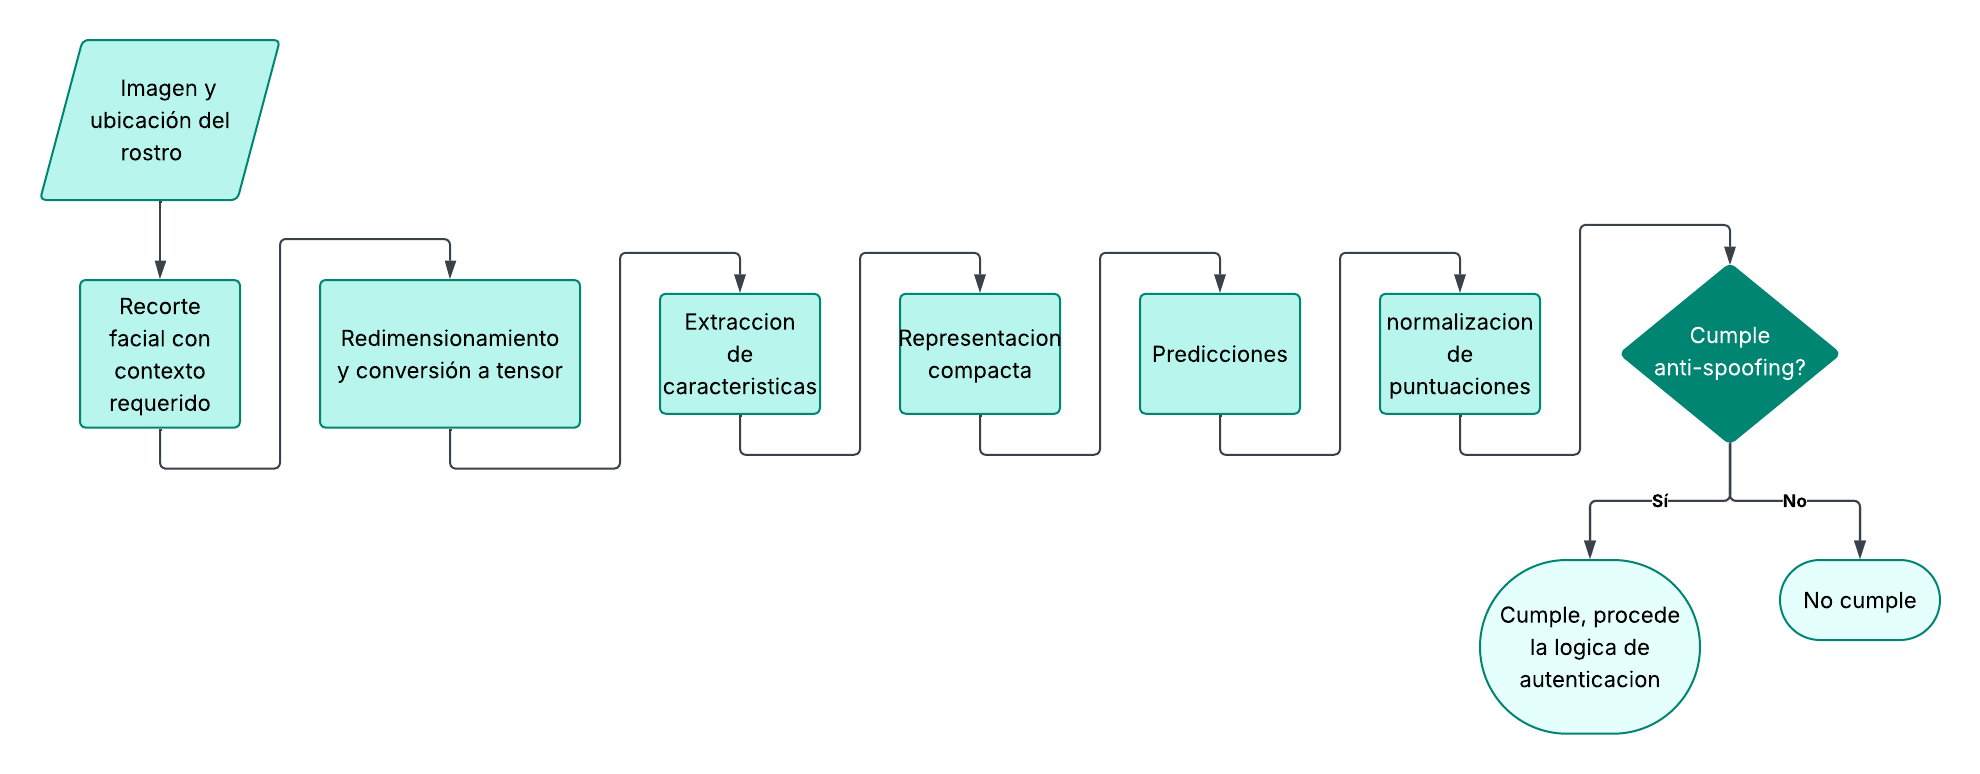
\includegraphics[width=\textwidth]{Imagenes/flujo_minifasnet.png}
    \caption{Diagrama de flujo de MiniFASNetV2.}
    \label{fig:flujo-minifasnet}
\end{figure}

\section{SFace: reconocimiento facial}

\subsection{Elección del modelo}

Se seleccionó SFace como modelo de reconocimiento facial de SmartGate para determinar la identidad del rostro que superó las etapas anteriores. A diferencia de un clasificador convencional, el modelo no genera directamente una clase correspondiente a cada usuario, sino una representación numérica de las características de la cara denominada \textit{embedding}.

Esta forma de representar los rostros resulta conveniente porque separa el modelo de reconocimiento de la cantidad concreta de usuarios registrados. Incorporar una nueva persona requiere obtener y almacenar su representación facial, en lugar de crear una nueva salida y volver a entrenar toda la red. Esto simplifica la administración de usuarios y permite actualizar el conjunto de personas autorizadas sin modificar el modelo.

Otro motivo de elección es que el entrenamiento mediante SFace busca obtener representaciones que permitan distinguir identidades, moderando la influencia de muestras problemáticas para reducir el sobreajuste a errores presentes en los datos de entrenamiento. Esta característica favorece la obtención de representaciones útiles para la comparación facial. La relación entre este entrenamiento y los vectores obtenidos se explica en el apartado de funcionamiento.

Además, la implementación disponible en OpenCV permite integrar la extracción de características y su comparación con el alineamiento basado en los cinco puntos faciales proporcionados por YuNet. Esta compatibilidad simplifica la conexión entre la detección y el reconocimiento, aprovechando información que ya se obtiene en una etapa anterior.

SFace constituye la última de las tres redes porque responde una pregunta que las etapas anteriores no resuelven. YuNet determina dónde se encuentra el rostro y MiniFASNetV2 evalúa su autenticidad, pero ninguno establece a quién pertenece. La combinación de los tres modelos permite así obtener de forma secuencial la localización, autenticidad e identidad necesarias para que la lógica de SmartGate tome la decisión final de acceso.

\subsection{Funcionamiento del modelo}

El flujo de reconocimiento comienza con el rostro que superó la comprobación de anti-spoofing. A partir de los puntos faciales obtenidos mediante YuNet, se realiza el alineamiento y el recorte de la imagen. Este procedimiento ajusta la posición, la escala y la inclinación del rostro en el plano de la imagen para que las muestras presenten una disposición comparable antes de ingresar a la red.

La imagen preparada se convierte al formato numérico de entrada requerido por el modelo. Esta conversión a tensor organiza los valores de los píxeles; todavía no constituye la generación del embedding. Posteriormente, la red convolucional procesa esos valores y extrae progresivamente características hasta producir un vector de longitud fija que representa información relevante para distinguir identidades.

En la versión distribuida por OpenCV, la red utilizada es MobileFaceNet, entrenada mediante la función de pérdida SFace. Durante el entrenamiento, esta función regula la aproximación de representaciones de una misma identidad y la separación de identidades diferentes. Para ello utiliza funciones sigmoides que moderan la contribución de las muestras al aprendizaje, buscando reducir el sobreajuste a datos problemáticos. Este procedimiento pertenece al entrenamiento previo y no se repite cada vez que SmartGate analiza un rostro.

Durante el uso del sistema, la salida de la red es el embedding de la muestra. La identificación se obtiene al compararlo con las representaciones almacenadas para los usuarios autorizados. Las muestras de registro deben prepararse y procesarse con el mismo modelo para que sus vectores sean comparables.

La comparación se realiza mediante una métrica. Con una métrica de similitud, los valores más altos indican una mayor semejanza; con una distancia, la mayor semejanza corresponde a valores más bajos. A partir de estas comparaciones se selecciona la mejor coincidencia y se comprueba si cumple el umbral de reconocimiento establecido.

Si la mejor coincidencia no cumple el umbral, la muestra se considera no reconocida, aunque exista un usuario cuyo vector sea el más cercano. Si lo cumple, se obtiene la identidad asociada a esa representación. Este resultado se entrega a la lógica de SmartGate, que lo utiliza junto con las comprobaciones anteriores y las condiciones de autorización para decidir el acceso.

\subsection{Diagrama de flujo del modelo}

\begin{figure}[H]
    \centering
    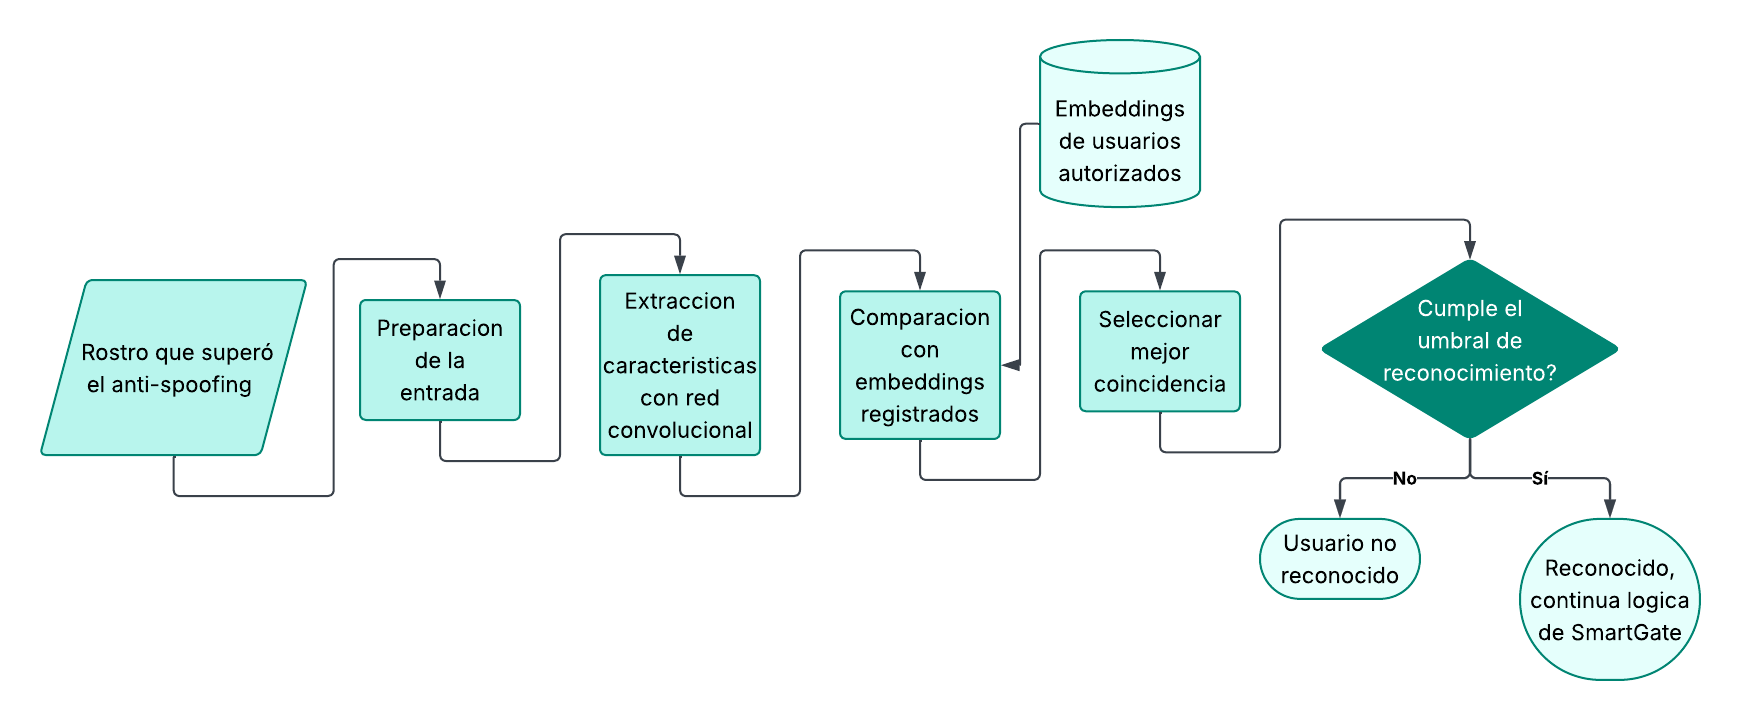
\includegraphics[width=\textwidth]{Imagenes/flujo_sface.png}
    \caption{Diagrama de flujo de SFace.}
    \label{fig:flujo-sface}
\end{figure}

\chapter{Programa en la Raspberry Pi}
\label{cap:programa}

\section{Estructura del programa}

El archivo \texttt{main.py} actúa como punto de entrada del sistema. Su función no es ejecutar directamente los modelos, sino preparar el entorno de trabajo: carga los parámetros de \texttt{config.yaml}, crea las señales y colas compartidas, inicializa los GPIO y pone en marcha los distintos workers. Cada worker se ejecuta en un hilo y permanece bloqueado mientras no tenga una tarea pendiente, lo que evita ciclos de consulta continua y reduce el uso innecesario del procesador.

Los principales hilos corresponden a detección, antispoofing, reconocimiento, telemetría, envío de eventos a Supabase y actualización de la galería facial. El control general queda a cargo del Pipeline Manager, que recibe mensajes de todos estos componentes y decide cuándo puede comenzar un nuevo ciclo, cuándo debe abrirse el portón y cómo recuperar un estado seguro ante un error o una apertura inesperada.

\section{Pipeline de procesamiento}

El procesamiento se organiza como una secuencia dirigida por eventos. Solamente se admite una persona dentro del pipeline en cada instante y la detección se habilita únicamente cuando el final de carrera indica que el portón está cerrado. De esta manera se evita procesar varios candidatos al mismo tiempo o iniciar una nueva autorización mientras el acceso se encuentra abierto.

El núcleo del sistema corresponde a la cadena cámara--detección--antispoofing--reconocimiento--decisión. La información avanza de forma ordenada por las siguientes etapas:

\begin{enumerate}
    \item La cámara conectada a la Raspberry Pi captura continuamente imágenes del entorno.
    \item YuNet localiza el rostro y obtiene los puntos de referencia necesarios para recortarlo y alinearlo.
    \item MiniFASNetV2 analiza la muestra para determinar si corresponde a una persona real o a un posible intento de suplantación.
    \item SFace genera un embedding facial que se compara con la galería de personas autorizadas.
    \item La lógica de decisión clasifica el intento como autorizado, desconocido o spoof y comunica el resultado al bloque de control físico.
\end{enumerate}

Cada una de estas etapas se describe a continuación.

\subsection{Detección del rostro}

La cámara Arducam OV5647, conectada mediante la interfaz CSI y administrada con Picamera2, entrega imágenes de $1280 \times 960$ píxeles. El primer worker utiliza YuNet para localizar un rostro y sus puntos de referencia. Cuando aparece un candidato con una confianza superior al umbral configurado, se deshabilita temporalmente la búsqueda de nuevas personas y se guardan dos muestras: un recorte ampliado para la comprobación de vida y la imagen original junto con los datos geométricos del rostro para el reconocimiento.

\subsection{Comprobación de persona}

La primera muestra es procesada por MiniFASNetV2. Este modelo determina si el rostro corresponde a una persona real o a un posible intento de suplantación, por ejemplo mediante una fotografía o una pantalla. Si el puntaje no supera el umbral de antispoofing, la segunda muestra se descarta, se registra un evento de tipo spoof y el sistema vuelve a habilitar la detección. Si la muestra es considerada real, se habilita la etapa de reconocimiento.

\subsection{Reconocimiento y decisión de acceso}

SFace alinea el rostro a partir de los puntos obtenidos por YuNet y genera un embedding. Se selecciona la mejor coincidencia y se comprueba que alcance el umbral configurado. Si no existe una coincidencia válida, la identidad se rechaza y el sistema vuelve al estado de espera.

Cuando la identidad es autorizada, el Pipeline Manager activa la señal luminosa correspondiente y genera un pulso de 500~ms sobre la salida que comanda la central del portón. A continuación espera que el final de carrera detecte primero la apertura y luego el cierre. Recién después de recuperar el estado de portón cerrado vuelve a habilitarse la detección de un nuevo usuario.

\begin{figure}[H]
    \centering
    \begin{tikzpicture}[node distance=1.3cm]
        \node[cajachica] (yunet) {\textbf{Cámara y YuNet}\\ Detección del rostro};
        \node[cajachica, below=of yunet] (fas) {\textbf{MiniFASNetV2}\\ Comprobación de vida};
        \node[cajachica, below=of fas] (sface) {\textbf{SFace}\\ Reconocimiento facial};
        \node[cajachica, below=of sface] (pm) {\textbf{Pipeline Manager}\\ Decisión, GPIO y portón};
        \node[cajachica, right=2.6cm of sface] (cache) {\textbf{Caché local}\\ IDs, nombres y embeddings};
        \node[cajachica, below=of cache] (supa) {\textbf{Supabase}\\ Usuarios y eventos};
        \draw[flecha] (yunet) -- node[etiqueta]{Candidato detectado} (fas);
        \draw[flecha] (fas) -- node[etiqueta]{Rostro validado} (sface);
        \draw[flecha] (sface) -- node[etiqueta]{Resultado del reconocimiento} (pm);
        \draw[dflecha] (sface) -- node[etiqueta]{Consulta de\\ galería facial} (cache);
        \draw[dflecha] (cache) -- node[etiqueta]{Sincronización} (supa);
    \end{tikzpicture}
    \caption{Pipeline principal ejecutado en la Raspberry Pi y relación con la galería facial.}
    \label{fig:pipeline-rpi}
\end{figure}

El diagrama presenta de forma simplificada las etapas principales del procesamiento y los componentes que intervienen en el reconocimiento. La galería facial almacenada localmente permite realizar las comparaciones sin depender de una consulta remota en cada intento de acceso. La sincronización con Supabase se ejecuta de manera independiente, mientras que el Pipeline Manager recibe los resultados de las distintas etapas y administra las decisiones del sistema.

\subsection{Integración de los modelos}

Los modelos se integraron mediante workers y buffers sincronizados. De esta forma cada etapa trabaja únicamente cuando la anterior produjo una muestra válida y el procesamiento más costoso no se ejecuta sobre todos los cuadros de la cámara. Esta organización también permite aislar errores y ajustar cada modelo sin reescribir el programa completo.

\begin{figure}[H]
    \centering
    % Reemplazar el recuadro por la imagen cuando esté disponible:
    % \includegraphics[width=\textwidth]{Imagenes/pipeline_smartgate.png}
    \fbox{\parbox[c][4cm][c]{0.9\textwidth}{\centering Imagen pendiente: \texttt{pipeline\_smartgate.png}}}
    \caption{Pipeline general implementado en SmartGate.}
    \label{fig:pipeline-general-smartgate}
\end{figure}

La figura~\ref{fig:pipeline-general-smartgate} reúne el camino principal de ejecución: captura y detección, validación de vida, reconocimiento, decisión del Pipeline Manager, control del portón, registro de eventos y sincronización con la página web y Supabase. También representa los buffers y colas utilizados para desacoplar los modelos y evitar que una operación de red bloquee la autorización.

Por claridad, el diagrama no muestra tres mecanismos auxiliares que forman parte de la implementación final. En primer lugar, systemd envuelve el proceso completo e inicia SmartGate al encender la Raspberry Pi (sección~\ref{sec:systemd}). En segundo lugar, la sincronización de rostros mantiene una galería local persistente en \texttt{data/galeria\_rostros.npz}; esta copia se carga antes de intentar conectarse a Supabase y permite reconocer usuarios durante una caída de red (sección~\ref{sec:offline}). Finalmente, si el Supabase Worker no puede enviar un evento, la cola se respalda en \texttt{data/eventos\_pendientes.jsonl} y se reenvía al recuperar la conexión (sección~\ref{sec:eventos}). Estos elementos completan el pipeline operativo aunque se hayan omitido de la figura para conservar su legibilidad.

\section{Concurrencia, estados y seguridad del flujo}

La coordinación entre los hilos se realiza con objetos \texttt{Event}, colas seguras y buffers compartidos. Las señales indican, entre otros estados, si el portón está cerrado, si la detección puede trabajar y si existe una muestra disponible para la siguiente etapa. Los modelos permanecen dormidos hasta recibir su evento, por lo que no compiten constantemente por los recursos de la placa.

El gestor emplea estados lógicos como \texttt{IDLE}, \texttt{PROCESSING}, \texttt{WAIT\_GATE\_OPEN}, \texttt{WAIT\_GATE\_CLOSE} y \texttt{CLEANING}. Si el portón se abre de manera inesperada o una etapa informa un error, se impide el ingreso de nuevos candidatos, se espera a que los tres modelos alcancen un punto seguro y se limpian los buffers antes de reanudar el servicio. Esta normalización evita que una imagen anterior quede asociada por error con el siguiente usuario.

El final de carrera se supervisa mediante \texttt{gpiod}. Un flanco ascendente representa que el portón dejó la posición de cerrado y un flanco descendente indica que volvió a cerrarse. Al arrancar, el nivel del pin se lee directamente, ya que todavía podría no haberse producido ningún flanco. Las funciones asociadas a estas interrupciones solamente actualizan el estado y notifican al gestor; las inferencias se mantienen fuera de la atención del GPIO.

\section{Arranque automático mediante systemd}
\label{sec:systemd}

systemd es el gestor de servicios utilizado por Raspberry Pi OS y otras distribuciones Linux. Se ejecuta durante el arranque del sistema operativo y se encarga de iniciar, detener y supervisar procesos definidos como servicios. En SmartGate se utilizó para que el programa comenzara a funcionar automáticamente cada vez que se encendiera la Raspberry Pi, sin necesidad de abrir una terminal ni ejecutar manualmente \texttt{main.py}.

La unidad \texttt{smartgate.service} se configuró como un servicio de tipo \texttt{simple}. En ella se define la carpeta de trabajo del proyecto y se indica que el comando de inicio es el script \texttt{systemd/iniciar\_smartgate.sh}. La opción \texttt{Restart=on-failure} solicita a systemd que vuelva a lanzar el programa si finaliza debido a un error, mientras que \texttt{RestartSec=5} introduce una espera de cinco segundos antes del reintento. Al quedar asociado a \texttt{default.target} y habilitado mediante \texttt{systemctl -{}-user enable smartgate.service}, el servicio se inicia automáticamente con la sesión del usuario.

El script de inicio espera hasta que Raspberry Pi OS haya creado un entorno gráfico Wayland o X11. Esta precaución evita que OpenCV intente utilizar la pantalla antes de que se encuentre disponible. Luego establece las variables \texttt{XDG\_RUNTIME\_DIR}, \texttt{WAYLAND\_DISPLAY} y \texttt{DISPLAY}, cambia a la carpeta del proyecto y utiliza \texttt{exec} para iniciar, sin procesos intermedios innecesarios, el intérprete del entorno virtual:

\begin{center}
\texttt{.venv/bin/python -u app/main.py}
\end{center}

La opción \texttt{-u} desactiva el almacenamiento temporal de la salida estándar, permitiendo observar inmediatamente los mensajes del programa en el registro del servicio. Para comprobar su estado pueden utilizarse \texttt{systemctl -{}-user status smartgate.service} y \texttt{journalctl -{}-user -u smartgate.service}. La figura~\ref{fig:systemd} resume el proceso completo.

\begin{figure}[H]
    \centering
    \begin{tikzpicture}[node distance=1.3cm]
        \node[caja] (on) {\textbf{Encendido}\\ Raspberry Pi OS};
        \node[caja, below=of on] (sd) {\textbf{systemd}\\ \texttt{smartgate.service}};
        \node[caja, below=of sd] (sc) {\textbf{Script de inicio}\\ Espera Wayland/X11};
        \node[caja, below=of sc] (venv) {\textbf{Entorno virtual}\\ \texttt{app/main.py}};
        \draw[flecha] (on) -- (sd);
        \draw[flecha] (sd) -- node[etiqueta]{ExecStart} (sc);
        \draw[flecha] (sc) -- node[etiqueta]{exec} (venv);
    \end{tikzpicture}
    \caption{Secuencia de arranque automático de SmartGate mediante systemd.}
    \label{fig:systemd}
\end{figure}

\chapter{Base de datos y funcionamiento sin conexión}
\label{cap:datos}

La persistencia remota de la información y una interfaz web que simplificara la administración de los usuarios se definieron como funcionalidades complementarias al MVP. Su implementación quedó condicionada al tiempo disponible luego de completar y validar el núcleo principal del sistema. Este capítulo describe cómo se resolvieron, junto con los mecanismos que permiten que el sistema siga funcionando cuando no hay conexión a Internet.

\section{Arquitectura de persistencia con Supabase}

Para esta etapa se utilizó el plan gratuito de Supabase, una plataforma que proporciona una base de datos PostgreSQL, almacenamiento de archivos y una API para acceder a los recursos del proyecto. En SmartGate, este servicio actúa como repositorio central: conserva los datos de las personas habilitadas, las representaciones faciales asociadas y los registros de acceso. Además, permite almacenar y recuperar las imágenes cargadas por los usuarios, manteniendo una copia persistente de la información disponible aun cuando la Raspberry Pi se reinicie o se encuentre temporalmente fuera de servicio.

La separación de la información en tablas facilita su mantenimiento. La tabla de personas contiene los datos identificatorios y el estado de habilitación; los vectores o características faciales se conservan de forma independiente; y los eventos generados por el sistema quedan registrados para su posterior consulta. Esta organización evita duplicaciones, mejora la trazabilidad y permite ampliar el sistema sin modificar la lógica principal de reconocimiento.

\section{Conexión con la Raspberry Pi}

La Raspberry Pi ejecuta el programa principal de SmartGate y se comunica con Supabase a través de su API mediante una conexión HTTPS. Al iniciarse, el software utiliza la dirección del proyecto y las credenciales configuradas localmente para consultar los usuarios habilitados y obtener las imágenes o representaciones faciales necesarias. Estos datos se descargan y quedan disponibles para el proceso de reconocimiento que se ejecuta en el dispositivo.

Durante el funcionamiento, la Raspberry Pi compara el rostro detectado con la información recuperada desde la base de datos. Si encuentra una coincidencia válida y el usuario está habilitado, la lógica del sistema continúa con la decisión de apertura. A su vez, los resultados de cada intento pueden enviarse nuevamente a Supabase como registros de acceso.

De este modo, la comunicación es bidireccional: la Raspberry Pi consume la información necesaria para reconocer a los usuarios y la base de datos recibe los eventos producidos por el sistema, tal como se muestra en la figura~\ref{fig:interaccion}.

\section{Interfaz web de administración}

Además de la base de datos, se desarrolló con asistencia de ChatGPT una interfaz web de administración. Su objetivo es ofrecer una capa visual sencilla para dar de alta o modificar usuarios, cargar imágenes y consultar los registros almacenados.

De esta manera, las tareas habituales pueden realizarse desde el navegador sin escribir consultas SQL ni ejecutar código, lo que reduce la posibilidad de errores y facilita el uso por parte de personas sin conocimientos técnicos.

La interfaz web presenta la información de forma centralizada. Desde el panel de control es posible consultar la cantidad de personas habilitadas, los accesos autorizados y rechazados, los eventos recientes y el estado general de los servicios. También se muestra explícitamente la conexión con Supabase, lo que facilita distinguir un problema de conectividad de una falla del pipeline local.

\begin{figure}[H]
    \centering
    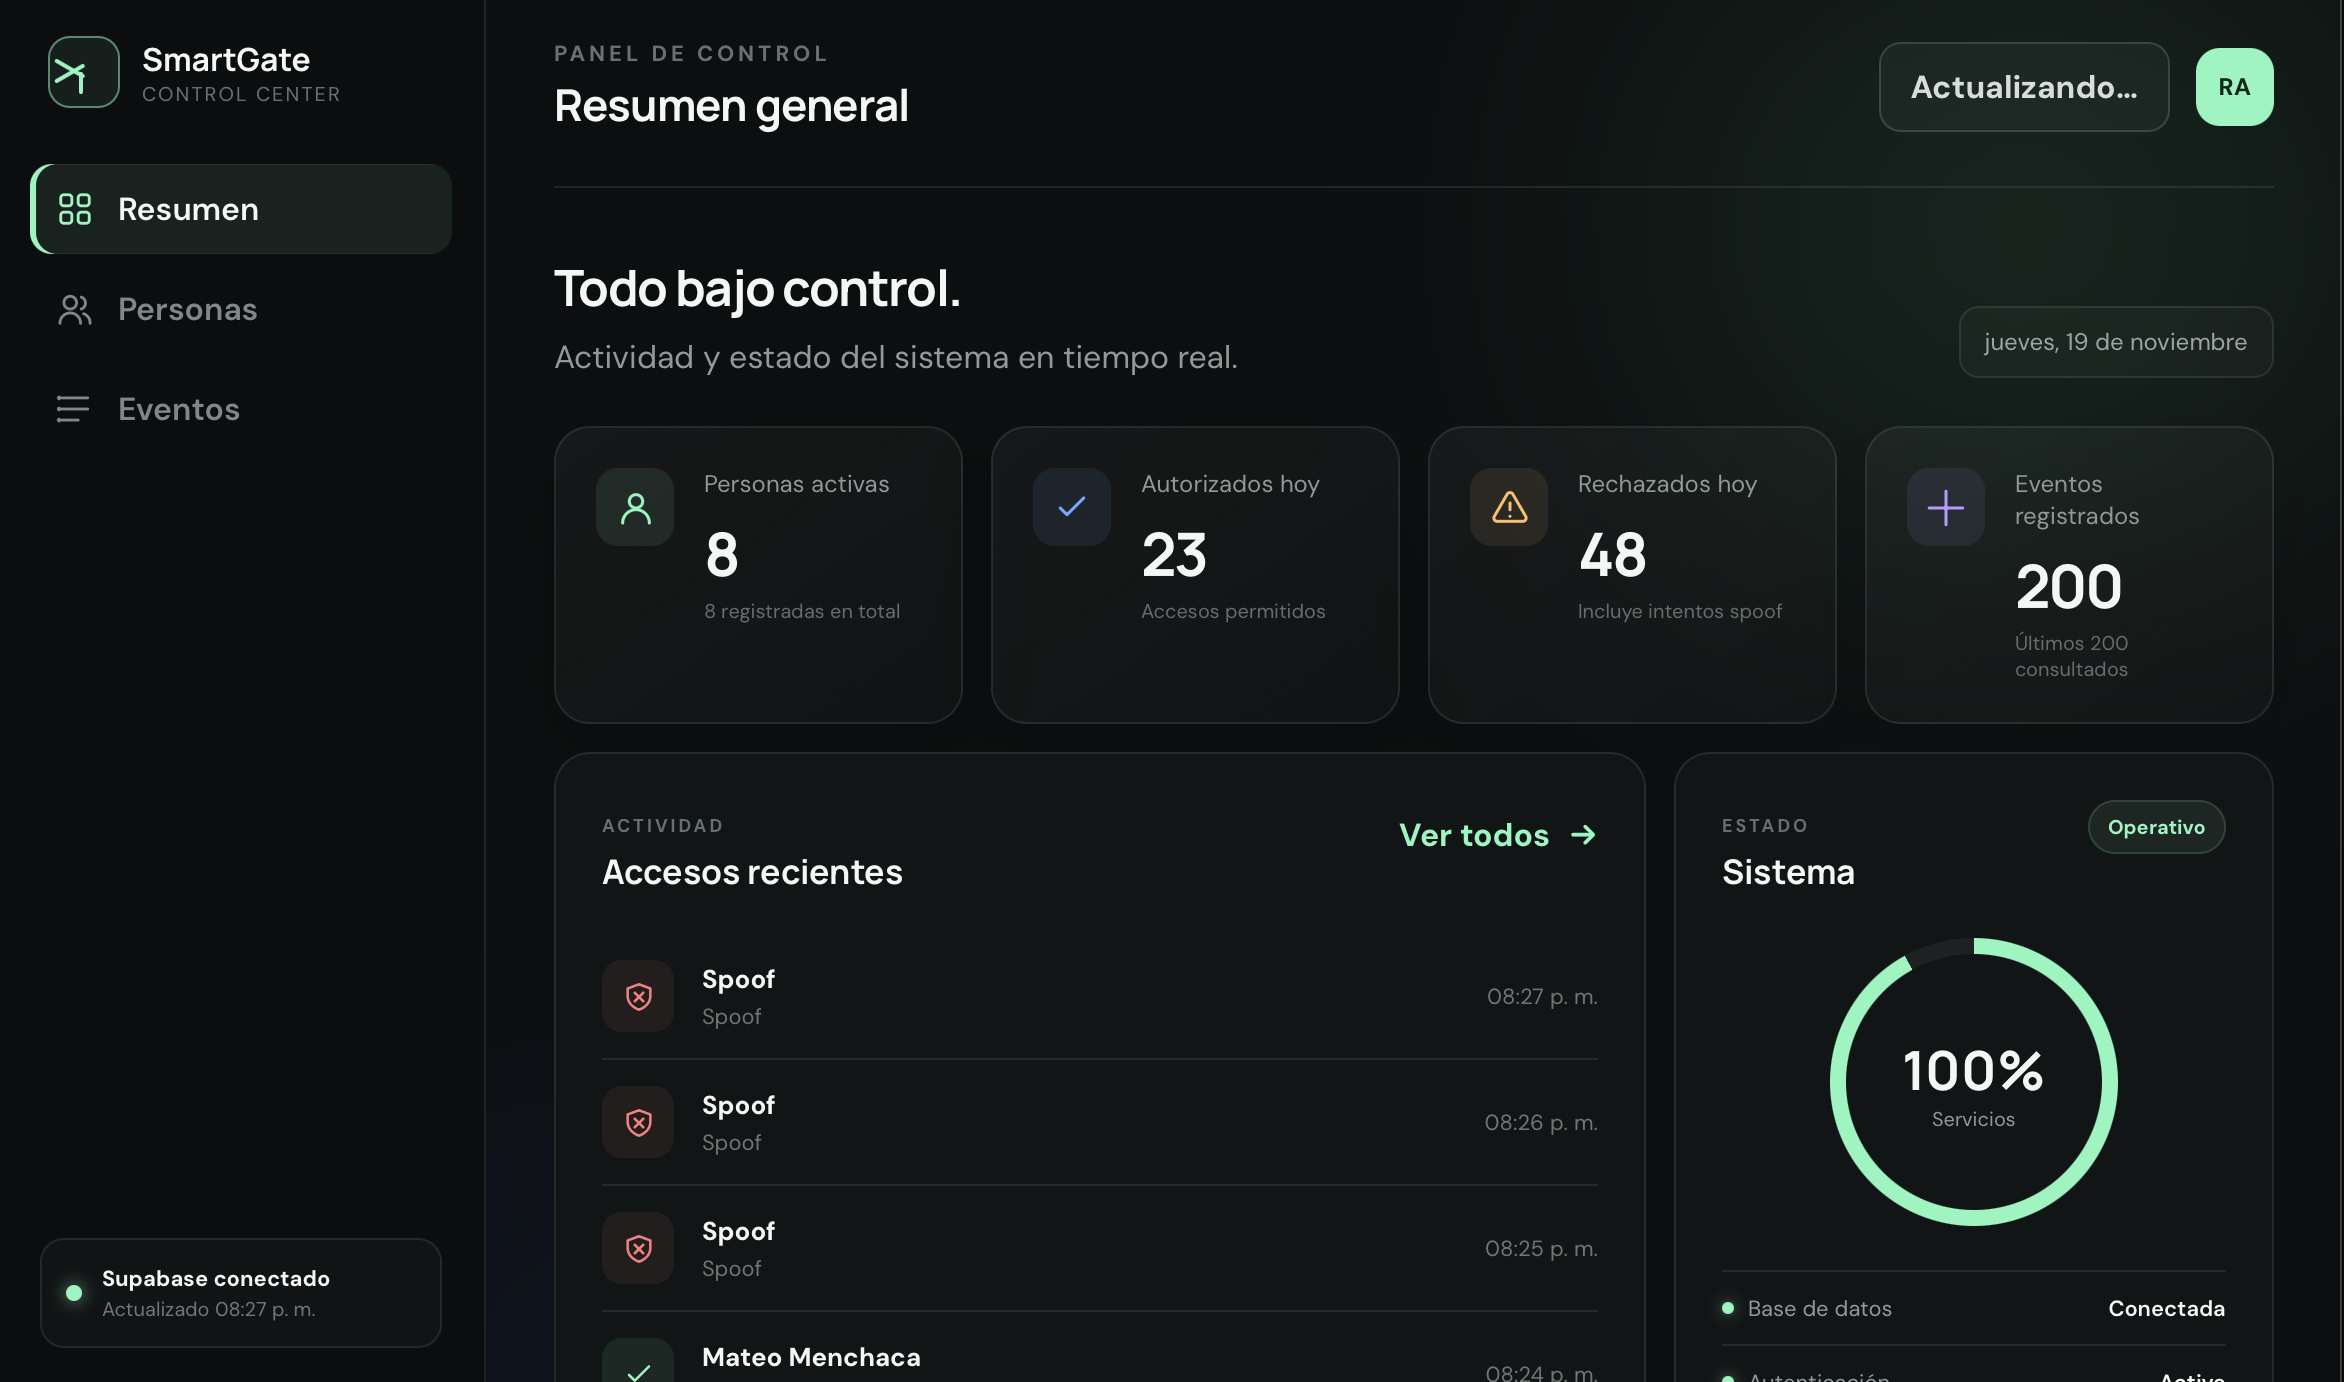
\includegraphics[width=\textwidth]{Imagenes/panel_web.png}
    \caption{Panel web de administración y supervisión conectado a Supabase.}
    \label{fig:panel-web}
\end{figure}

La vista de eventos permite revisar rápidamente resultados autorizados, rechazados y clasificados como spoof. De esta manera, Supabase no solamente cumple una función de almacenamiento, sino que también aporta trazabilidad y una capa de supervisión para evaluar el comportamiento del sistema durante las pruebas.

Como criterio de seguridad, las claves privadas de acceso no deben incorporarse al código visible de la interfaz web. Estas credenciales deben mantenerse en la Raspberry Pi o en un servicio de servidor, mientras que la aplicación web debe operar únicamente con permisos limitados y las políticas de acceso definidas en Supabase.

\section{Funcionamiento sin conexión}
\label{sec:offline}

La conectividad con Supabase se ejecuta en hilos independientes y nunca forma parte del camino crítico de autorización. Por esta razón, una red lenta o la ausencia de Wi-Fi no detienen la cámara, los modelos ni el control GPIO. Para que el reconocimiento pueda continuar, el sistema mantiene en la tarjeta de la Raspberry una copia de la última galería facial válida.

\subsection{Galería facial local}

Aunque habitualmente se la denomina caché de imágenes, el archivo local no conserva las fotografías completas. Durante la sincronización, las imágenes alojadas en Supabase se descargan, se validan y se transforman en embeddings de 128 valores. El respaldo \texttt{data/galeria\_rostros.npz} almacena de forma compacta el identificador, el nombre y los embeddings de cada persona habilitada. Esta representación es suficiente para realizar las comparaciones de SFace y reduce tanto el espacio utilizado como el tiempo de carga.

Al comenzar el reconocimiento, el programa carga primero esta galería desde el disco, antes de intentar comunicarse con Supabase. Por lo tanto, si la placa arranca sin Wi-Fi puede reconocer inmediatamente a los usuarios incluidos en la última sincronización. En paralelo, el worker de galería intenta recuperar la conexión cada diez segundos. Cuando Supabase vuelve a estar disponible, obtiene las personas activas y sus embeddings, compara la nueva galería con la existente y solamente escribe el archivo si hubo cambios.

El guardado de la galería se realiza de forma atómica: se genera un archivo temporal, se fuerza su escritura en la tarjeta y finalmente se reemplaza la versión anterior. De este modo, un corte de alimentación durante la actualización no debería dejar un respaldo incompleto. Además, la galería compartida en memoria se protege mediante un \texttt{Lock}, por lo que puede actualizarse sin interrumpir un reconocimiento que ya se encuentre en curso.

Durante el modo sin conexión se cumplen las siguientes condiciones:

\begin{itemize}
    \item Los usuarios presentes en la última galería sincronizada pueden continuar ingresando.
    \item Las altas, bajas, cambios de habilitación y fotografías nuevas no se reciben hasta recuperar la conexión.
    \item El funcionamiento offline requiere que haya existido al menos una sincronización válida anterior.
    \item Si no existe una galería local, el pipeline puede ejecutarse, pero no tendrá identidades contra las cuales comparar el rostro.
\end{itemize}

\subsection{Persistencia de los eventos de acceso}
\label{sec:eventos}

Los resultados autorizados, rechazados o clasificados como spoof se colocan en una cola en memoria para que el Pipeline Manager pueda continuar sin esperar una respuesta de Internet. Un worker separado intenta insertarlos en la tabla \texttt{access\_events}. Si el envío falla, cada evento se agrega como una línea JSON al archivo \texttt{data/eventos\_pendientes.jsonl}.

Mientras la placa permanezca desconectada, los eventos se acumulan en ese archivo. El worker vuelve a intentar la conexión periódicamente y, cuando la recupera, envía primero los eventos antiguos respetando su orden y después los nuevos. Los registros confirmados se eliminan del respaldo local; si una transferencia vuelve a fallar, se conserva el evento problemático junto con todos los posteriores. Así se mantiene la trazabilidad sin bloquear la decisión de acceso.

En conjunto, esta estrategia combina procesamiento local, caché persistente y sincronización diferida. Supabase permite administrar usuarios y centralizar los registros, pero la operación física del portón permanece disponible aun frente a una interrupción temporal de la red.

\chapter{Desarrollo, pruebas y resultados}
\label{cap:desarrollo}

\section{Desarrollo e implementación del MVP}

El MVP se definió como el conjunto mínimo de componentes necesarios para reconocer a una persona autorizada, descartar intentos básicos de suplantación y accionar el acceso físico. Su objetivo no era ofrecer desde el inicio todas las funciones de administración o conectividad, sino validar que el sistema pudiera completar el ciclo principal de forma autónoma sobre la Raspberry Pi.

\subsection{Pipeline de visión y decisión}

El núcleo del MVP corresponde a la cadena cámara--detección--antispoofing--reconocimiento--decisión descrita en el capítulo~\ref{cap:programa}. Se construyó primero con modelos previamente entrenados, integrados mediante workers y buffers sincronizados.

\subsection{Control físico y funcionamiento local}

Una vez validado el pipeline de visión, se incorporaron las entradas y salidas GPIO, la señalización luminosa, el pulso de apertura y la lectura del final de carrera. El ciclo del MVP quedó completo cuando la Raspberry Pi pudo detectar al usuario, validar su identidad, indicar el resultado, accionar la central del portón y esperar su apertura y cierre antes de habilitar un nuevo intento.

El procesamiento principal se ejecuta localmente. Por lo tanto, la decisión de acceso no depende de enviar cada imagen a un servidor externo. Esta característica reduce la latencia y mantiene el funcionamiento básico aun cuando la conexión a Internet no se encuentra disponible, siempre que exista una galería local previamente sincronizada.

\subsection{Resultado del MVP}

Al finalizar esta etapa quedaron implementados los siguientes componentes:

\begin{itemize}
    \item Adquisición de imágenes desde la cámara.
    \item Detección, comprobación de vida y reconocimiento facial.
    \item Comparación contra una galería local de usuarios.
    \item Decisión de acceso y clasificación de intentos de suplantación.
    \item Señalización de los estados activo, procesando, aceptado y rechazado.
    \item Accionamiento de la central del portón y supervisión del final de carrera.
    \item Registro básico del resultado de cada intento.
\end{itemize}

Estos elementos forman el núcleo indispensable de SmartGate. Las funciones desarrolladas posteriormente amplían la administración, la trazabilidad y la robustez.

\section{Pruebas con personas y errores observados}

Para evaluar el comportamiento real del sistema se realizaron pruebas repetidas con distintas personas. Los ensayos buscaron observar tanto falsos positivos como falsos negativos en las etapas de detección, antispoofing y reconocimiento, incluyendo usuarios registrados y personas que no formaban parte de la galería autorizada.

En el conjunto de pruebas efectuado se registró una única clasificación incorrecta. El error estuvo asociado al módulo de antispoofing y no a la comparación de identidad realizada por SFace. Considerando que los modelos utilizados no habían sido entrenados específicamente con imágenes obtenidas en el entorno de SmartGate, obtener un solo error después de probar el sistema con varias personas representó un resultado muy favorable para el prototipo.

Estas pruebas también reforzaron la utilidad del entrenamiento que había sido planificado como extra. Un conjunto de datos propio, con ejemplos capturados por la cámara definitiva y bajo las condiciones reales de iluminación, distancia y pose, habría permitido ajustar especialmente el antispoofing y posiblemente reducir todavía más este tipo de error. Sin embargo, al no contarse con una cantidad suficiente de muestras, los resultados deben interpretarse como una validación funcional y no como una medición estadística definitiva de la tasa de falsos positivos o falsos negativos.

\section{Funcionalidades adicionales}

\subsection{Extras implementados}

Una vez estabilizado el MVP se incorporaron las funcionalidades adicionales priorizadas para el proyecto, descritas en los capítulos~\ref{cap:programa} y~\ref{cap:datos}:

\begin{itemize}
    \item La base de datos de Supabase permitió centralizar usuarios, embeddings y eventos de acceso, mientras que la interfaz web simplificó las altas, bajas y cambios de habilitación. También se agregó la sincronización periódica de la galería sin interrumpir el reconocimiento en curso.
    \item Para evitar que una interrupción de red detuviera el sistema se desarrolló una caché local persistente con la última galería válida y un archivo de eventos pendientes. Cuando no hay conexión, la placa continúa reconociendo a los usuarios almacenados localmente y conserva los nuevos eventos. Al recuperar Internet, envía primero los registros acumulados y luego continúa con los eventos nuevos.
    \item También se configuró systemd para iniciar el programa automáticamente al encender la Raspberry Pi, reiniciarlo ante fallos y facilitar la consulta de su estado.
\end{itemize}

Junto con la modularización, la telemetría y el manejo de errores, estas funciones mejoran la autonomía necesaria para un dispositivo que debe operar sin intervención constante.

\subsection{Herramienta para la construcción del dataset}

Como parte del extra asociado a modelos propios se desarrolló un script de adquisición de datos. El programa levantaba un servidor local en un puerto de la computadora y ofrecía una interfaz accesible desde el navegador. Desde esa interfaz era posible completar los metadatos definidos para cada muestra y controlar la toma de fotografías. Las imágenes y su información asociada se guardaban de forma organizada para formar el dataset que posteriormente se utilizaría durante el entrenamiento.

Esta herramienta permitía estandarizar la recolección y reducir errores de identificación o clasificación manual. Además, dejaba preparada una base reutilizable para continuar capturando datos con distintas personas y condiciones de iluminación, distancia, pose y presentación frente a la cámara.

Sin embargo, durante el período del proyecto no se alcanzó la cantidad mínima ni la diversidad de fotografías necesarias para realizar un entrenamiento confiable. Utilizar un conjunto demasiado pequeño habría producido resultados poco representativos y un riesgo elevado de sobreajuste. Por ese motivo no se consideró correcto presentar un modelo entrenado con datos insuficientes como una mejora válida del sistema.

\subsection{Proceso de entrenamiento iniciado}

En paralelo con la captura se comenzó a desarrollar el proceso de entrenamiento: preparación y lectura del dataset, asociación de imágenes con sus metadatos y definición del flujo necesario para entrenar y validar los modelos. Esta etapa avanzó a nivel de infraestructura y procedimiento, pero no pudo culminarse porque el dataset todavía no tenía el volumen requerido y el tiempo restante no permitía completar una nueva campaña de adquisición, ejecutar los experimentos y validar los resultados.

Por lo tanto, el único extra priorizado que quedó incompleto fue el entrenamiento o ajuste profundo de modelos específicamente para SmartGate. La versión final utiliza modelos previamente entrenados y umbrales ajustados durante las pruebas. La herramienta de captura y el trabajo inicial del pipeline de entrenamiento constituyen un avance aprovechable para una etapa posterior, pero no se contabilizan como un modelo propio finalizado.

\section{Separación entre MVP y extras}

La tabla~\ref{tab:mvp-extras} resume qué bloques forman parte del MVP y cuáles corresponden a funcionalidades adicionales, junto con el resultado alcanzado en cada uno.

\begin{table}[H]
    \centering
    \small
    \renewcommand{\baselinestretch}{1.15}\selectfont
    \begin{tabular}{|p{4.0cm}|p{4.0cm}|p{6.1cm}|}
        \hline
        \textbf{Bloque} & \textbf{Función dentro del proyecto} & \textbf{Resultado} \\ \hline
        Pipeline de visión & Detección, antispoofing, reconocimiento y decisión & MVP completado con modelos previamente entrenados. \\ \hline
        Control físico & Señalización, pulso de apertura y lectura del final de carrera & MVP completado e integrado con el pipeline. \\ \hline
        Persistencia local básica & Galería disponible para tomar la decisión de acceso & Parte del funcionamiento autónomo del MVP. \\ \hline
        Supabase e interfaz web & Administración centralizada de usuarios y eventos & Extra implementado. \\ \hline
        Caché offline y sincronización diferida & Continuidad sin red y envío posterior de eventos & Extra implementado. \\ \hline
        systemd, telemetría y recuperación & Arranque automático y mayor autonomía operativa & Extra implementado. \\ \hline
        Captura del dataset & Interfaz local para fotografías y metadatos & Herramienta implementada; dataset insuficiente. \\ \hline
        Entrenamiento de modelos propios & Adaptación a las condiciones reales de SmartGate & Proceso iniciado, pero no culminado. \\ \hline
    \end{tabular}
    \caption{Separación entre el MVP y las funcionalidades adicionales.}
    \label{tab:mvp-extras}
\end{table}

\section{Repositorio del proyecto}

Todo el desarrollo correspondiente al núcleo de SmartGate se mantuvo versionado en el repositorio de GitHub del proyecto, disponible en \url{https://github.com/ms282489/SmartGate}. El repositorio permite observar la evolución del sistema a través de los tres prototipos desarrollados, desde las primeras pruebas individuales de los modelos hasta la integración del pipeline, el control físico, la telemetría y la comunicación con la base de datos. También se conserva la documentación utilizada para definir la arquitectura y lógica de funcionamiento, junto con los programas desarrollados para la adquisición de imágenes y generación de datasets.

La obtención de un dataset propio fue más limitada de lo previsto, por lo que en el repositorio se priorizó conservar las herramientas, configuraciones y metodología de captura desarrolladas. Las imágenes obtenidas no se almacenaron directamente en GitHub debido tanto a su volumen como al carácter biométrico de la información. De esta forma, el repositorio documenta el procedimiento utilizado para generar y organizar las muestras sin publicar los datos faciales adquiridos.

La interfaz web de administración constituye la principal parte del desarrollo que no se encuentra almacenada dentro de este repositorio. Esta funcionalidad fue desarrollada de forma desacoplada del software ejecutado en la Raspberry Pi, al tratarse de una prestación complementaria incorporada posteriormente al MVP. La comunicación entre ambos desarrollos se realiza mediante Supabase, que actúa como repositorio central para la información de usuarios, representaciones faciales y registros de acceso. Dentro del repositorio de SmartGate sí se encuentran los módulos implementados en la Raspberry Pi para realizar esta sincronización, pero no el código correspondiente a la interfaz web administrativa.

\chapter{Planificación y cumplimiento}

\section{Diagrama de Gantt}

El diagrama de Gantt del anteproyecto organizaba el trabajo en una etapa de investigación, dos iteraciones de desarrollo, entregas intermedias, pruebas intensivas, documentación y un período final para extras. La primera iteración concentraba el pipeline, la configuración de la Raspberry Pi, el hardware base, el control físico y la integración inicial. La segunda contemplaba los ajustes de la primera versión y, si el tiempo lo permitía, la mejora y el entrenamiento de modelos.

\begin{figure}[H]
    \centering
    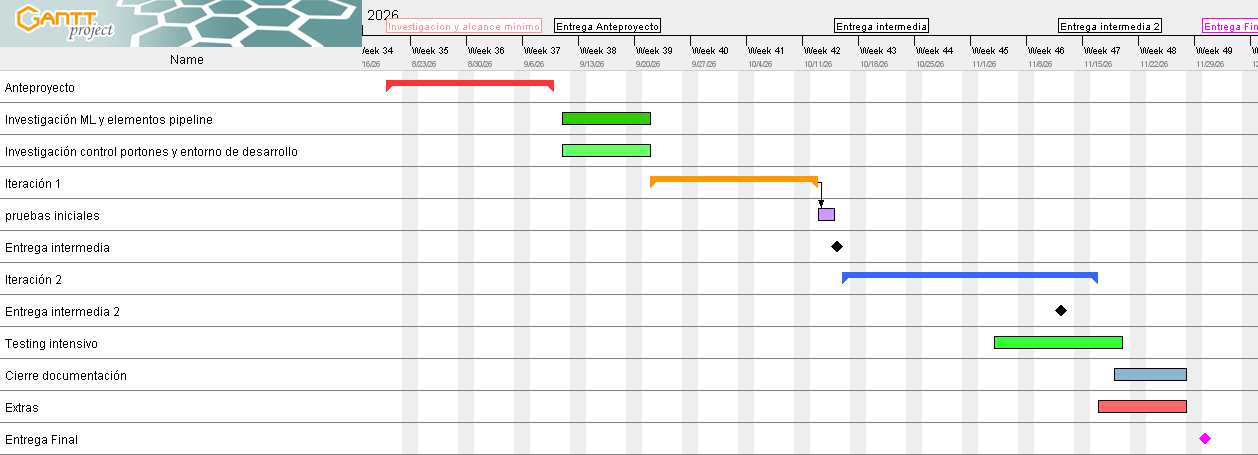
\includegraphics[width=\textwidth]{Imagenes/gantt_anteproyecto.png}
    \caption{Diagrama de Gantt del anteproyecto.}
    \label{fig:gantt}
\end{figure}

Al comparar el desarrollo realizado con el diagrama de Gantt definido al comienzo del proyecto, la planificación general pudo respetarse en buena medida. Las etapas de investigación, desarrollo de los prototipos, integración, pruebas y cierre de documentación se mantuvieron aproximadamente dentro de los períodos previstos, aunque algunas actividades debieron ejecutarse en paralelo o modificarse en función de los resultados obtenidos durante el desarrollo.

\section{Comparación con lo planificado}

La tabla~\ref{tab:cumplimiento-gantt} compara cada etapa planificada con el resultado obtenido.

\begin{table}[H]
    \centering
    \small
    \renewcommand{\baselinestretch}{1.15}\selectfont
    \begin{tabular}{|p{3.5cm}|p{2.4cm}|p{7.9cm}|}
        \hline
        \textbf{Etapa planificada} & \textbf{Resultado} & \textbf{Observaciones} \\ \hline
        Investigación y anteproyecto & Cumplida & Se definieron el alcance, la arquitectura, la plataforma y los modelos iniciales. \\ \hline
        Iteración 1 e integración del MVP & Cumplida & Se desarrollaron el pipeline, la Raspberry Pi, el control físico y las pruebas iniciales. \\ \hline
        Ajustes de la segunda iteración & Cumplida & Se modularizó el programa y se mejoró la sincronización, el manejo de estados y la recuperación ante errores. \\ \hline
        Extras operativos & Cumplida & Se implementaron Supabase, interfaz web, caché offline, eventos pendientes y systemd. \\ \hline
        Construcción del dataset & Cumplida parcialmente & Se desarrolló la herramienta de captura y se tomaron muestras, pero no se alcanzó el volumen mínimo necesario. \\ \hline
        Entrenamiento específico & No culminada & El proceso comenzó, pero la falta de datos suficientes y de tiempo impidió entrenar y validar modelos propios. \\ \hline
        Pruebas y documentación & Cumplida & Se probaron el pipeline, la cámara, el GPIO, la base de datos y el modo offline, y se consolidó el informe. \\ \hline
    \end{tabular}
    \caption{Comparación entre la planificación del Gantt y el resultado final.}
    \label{tab:cumplimiento-gantt}
\end{table}

\section{Desvíos respecto de la planificación}

\subsection{Base de datos e interfaz web en paralelo}

Una de las principales diferencias respecto a la planificación fue la incorporación de la base de datos y de la interfaz web de administración. Estas funcionalidades habían sido planteadas inicialmente como prestaciones adicionales posteriores al cumplimiento del MVP; sin embargo, se decidió avanzar sobre ellas en paralelo al desarrollo principal. Esto permitió integrar Supabase con el sistema y disponer de una gestión más completa de usuarios y registros sin desplazar como prioridad el funcionamiento del pipeline y del control de acceso.

\subsection{Entrenamiento propio no realizado}

El desvío principal respecto a lo planificado se concentró en el entrenamiento propio. No se llegó a realizar el entrenamiento o ajuste específico de los modelos con un dataset propio, previsto como una posible mejora durante la segunda iteración. Esta tarea resultó considerablemente más ambiciosa de lo estimado inicialmente, principalmente por la cantidad y diversidad de muestras necesarias para obtener resultados representativos dentro del tiempo disponible.

No se trataba de una condición para validar el MVP, ya que desde el anteproyecto se admitía el uso de modelos previamente entrenados. Frente al tiempo disponible se priorizó completar la integración, probar el sistema de extremo a extremo y dejar una base de captura y entrenamiento que pudiera continuarse posteriormente.

\subsection{Disponibilidad del hardware}

A esta limitación se sumaron dificultades externas en la obtención del hardware. Si bien el equipo disponía inicialmente de una placa de desarrollo, durante una parte importante del proyecto no se contó con una cámara adecuada, lo que imposibilitó comenzar tempranamente las pruebas reales de adquisición de imágenes y la generación del dataset. La disponibilidad de los componentes dependió de compras y envíos externos, por lo que este retraso no podía resolverse directamente desde el equipo de proyecto ni desde el equipo docente. Una vez disponible el hardware necesario, se priorizaron las pruebas del pipeline completo, la integración entre módulos y la validación del MVP.

En consecuencia, aunque fue necesario adaptar algunas de las actividades previstas, se conservaron los principales hitos y objetivos temporales del cronograma. Las desviaciones se concentraron principalmente en funcionalidades adicionales y en el entrenamiento específico de modelos, mientras que el esfuerzo final se orientó a asegurar la implementación e integración de las funciones consideradas esenciales para SmartGate.

\chapter{Alcance, limitaciones y trabajo futuro}

\section{Alcance actual y limitaciones}

El prototipo demuestra que es posible integrar visión artificial, procesamiento local, control físico y servicios remotos en una plataforma de costo moderado. También demuestra continuidad operativa ante interrupciones temporales de Internet y la posibilidad de administrar los usuarios desde una interfaz independiente de la Raspberry Pi.

La limitación práctica más visible se encuentra en la adquisición de imagen. La cámara utilizada permite validar el sistema a corta distancia, pero cuando la persona se aleja el rostro ocupa pocos píxeles. En esas condiciones la detección y la extracción de características se vuelven menos estables, por lo que actualmente el usuario debe aproximarse para ser reconocido. La iluminación, el contraluz, el ángulo de montaje y el movimiento también influyen en las etapas posteriores.

Esta limitación no depende únicamente del modelo. Un entrenamiento adaptado puede aumentar la robustez, pero no puede recuperar información que la cámara no capturó. Por ello, el sistema todavía debe considerarse un prototipo funcional y no una solución de seguridad definitiva. Antes de un despliegue continuo sería necesario ampliar las pruebas, medir falsas aceptaciones y falsos rechazos, reforzar la protección de credenciales y datos biométricos y definir procedimientos de mantenimiento y contingencia.

\section{Alcance potencial y trabajo futuro}

El siguiente paso natural es completar el dataset mediante la herramienta ya desarrollada. La campaña de captura debería incluir una cantidad suficiente de personas y variaciones de iluminación, distancia, orientación, expresión, accesorios y posibles ataques de suplantación. Con esos datos podría retomarse el pipeline de entrenamiento, separar conjuntos de entrenamiento y validación y calibrar los umbrales con métricas objetivas.

En el hardware podría incorporarse una cámara con mayor resolución efectiva sobre el rostro, mejor comportamiento con poca luz o una óptica adecuada a la distancia de operación. Una iluminación frontal controlada y una ubicación de montaje correctamente estudiada también permitirían detectar al usuario desde una posición más cómoda. Si se requiriera mayor velocidad, modelos más complejos o varias cámaras, podría añadirse aceleración dedicada para inferencia o una plataforma de procesamiento de mayores prestaciones.

La arquitectura de datos permite ampliar el proyecto hacia permisos por horario, diferentes niveles de autorización, múltiples puntos de acceso, auditoría centralizada y supervisión remota. La interfaz web podría incorporar estadísticas, alertas y herramientas de diagnóstico. Estas ampliaciones deberían acompañarse de políticas de acceso, cifrado, copias de seguridad y protección específica de los datos biométricos.

En síntesis, el desarrollo escalonado permitió completar el MVP y la mayor parte de los extras operativos. El único objetivo adicional no culminado fue el entrenamiento de modelos propios: se construyó la herramienta de captura, se inició la recolección del dataset y se comenzó el proceso de entrenamiento, pero no se alcanzaron los datos ni el tiempo necesarios para obtener y validar un modelo confiable. Este trabajo deja una base concreta para continuar la evolución de SmartGate sin modificar la arquitectura principal.

\chapter{Conclusión}

El desarrollo de SmartGate permitió cumplir con el objetivo principal del proyecto: implementar un sistema de control de acceso mediante reconocimiento facial, capaz de realizar el procesamiento y la toma de decisiones de forma local sobre una Raspberry Pi. La integración de los modelos de detección facial, antispoofing y reconocimiento, junto con la electrónica de control del portón, permitió obtener un prototipo funcional que reúne las características definidas para el producto mínimo viable (MVP).

Uno de los principales resultados fue demostrar la viabilidad de ejecutar múltiples modelos de machine learning sobre una plataforma embebida de recursos limitados, sin recurrir a aceleradores especializados ni depender de servicios externos para realizar las inferencias. La arquitectura modular y el procesamiento basado en eventos permitieron coordinar las distintas etapas, administrar los recursos disponibles y mantener un funcionamiento ordenado frente a cambios de estado del portón o errores durante la ejecución.

Además del cumplimiento del MVP, se logró incorporar gran parte de las funcionalidades complementarias previstas. La integración con Supabase, la interfaz web de administración, la persistencia local y los mecanismos de sincronización permitieron ampliar considerablemente las capacidades del sistema. Estas implementaciones aportaron autonomía, trazabilidad y facilidad de administración, manteniendo la posibilidad de operar ante interrupciones temporales de conectividad.

Las pruebas realizadas con distintas personas permitieron comprobar el funcionamiento conjunto de los módulos y obtener resultados favorables para esta etapa de desarrollo. Sin embargo, también se identificaron limitaciones relacionadas principalmente con las condiciones de captura de imágenes y la capacidad de generalización de los modelos utilizados. El entrenamiento específico con un dataset propio no pudo completarse debido al tiempo disponible y a las dificultades encontradas durante la adquisición de muestras, aunque se desarrollaron herramientas que permitirán retomar esta tarea posteriormente.

Desde el punto de vista de la planificación, las principales etapas y entregas pudieron mantenerse dentro de los plazos establecidos, adaptando las prioridades frente a las dificultades de disponibilidad de hardware y a la complejidad de determinadas funcionalidades. Esta experiencia evidenció la importancia de establecer objetivos alcanzables, desarrollar de forma incremental y validar progresivamente cada módulo antes de avanzar hacia una integración completa.

En definitiva, SmartGate constituye una implementación funcional que demuestra la posibilidad de combinar visión artificial, sistemas embebidos, diseño electrónico y servicios de administración remota en una solución de control de acceso. Si bien todavía requiere una validación más extensa y mejoras para su utilización en un entorno real de manera permanente, el desarrollo alcanzado establece una base técnica sólida y ampliable, sobre la cual es posible continuar optimizando el reconocimiento, la seguridad y las prestaciones generales del sistema.


\begin{thebibliography}{9}

\bibitem{ppa-triflex} PPA -- Motoppar Indústria e Comércio de Automatizadores Ltda., \textit{Central Triflex Facility -- Manual Técnico}, Rev. 4, P05634, 2022. Documentación técnica de la central, conexiones de botonera, alimentación auxiliar y sensores reed de final de carrera.

\bibitem{ppa-pop} PPA -- Motoppar Indústria e Comércio de Automatizadores Ltda., \textit{Central Agility Pop Connect -- Manual de instrucciones}. Documentación técnica de la central, entrada de botonera, final de carrera analógico y fuente interna de 12~V.

\bibitem{seg-wave} SEG, \textit{Central Wave -- Manual de instrucciones}. Documentación de entradas de botonera, finales de carrera, función condominio y salida auxiliar de 12~V.

\bibitem{seg-g2} SEG, \textit{Central G-II Mono -- Manual de Instalación}, versión 2.3. Documentación de botoneras, finales de carrera y salida auxiliar de 12~Vcc/400~mA no regulada.

\bibitem{seg-solo} SEG, \textit{Solo CH -- Manual de Instalación}. Documentación del automatizador y utilización de sensores magnéticos reed normalmente abiertos para los finales de carrera.

\bibitem{yunet} W. Wu, H. Peng y S. Yu, \textit{YuNet: A Tiny Millisecond-level Face Detector}, Machine Intelligence Research, vol. 20, pp. 656--665, 2023. Descripción de la arquitectura YuNet y su aplicación en sistemas con recursos computacionales limitados.

\bibitem{opencv} OpenCV, \textit{DNN-based Face Detection and Recognition}. Documentación de los modelos YuNet y SFace, detección facial, puntos de referencia, alineamiento, extracción de características y comparación mediante similitud coseno y distancia L2.

\bibitem{minivision} MiniVision AI, \textit{Silent-Face-Anti-Spoofing}. Implementación de MiniFASNetV2 para la detección de ataques de suplantación facial y clasificación de muestras reales y falsas.

\bibitem{cdcn} Z. Yu et al., \textit{Searching Central Difference Convolutional Networks for Face Anti-Spoofing}, IEEE/CVF Conference on Computer Vision and Pattern Recognition, 2020.

\end{thebibliography}

\end{document}
